%%
%% Copyright 2025 Oxford University Press
%%
%% This file is part of the 'oup-authoring-template Bundle'.
%% ---------------------------------------------
%%
%% It may be distributed under the conditions of the LaTeX Project Public
%% License, either version 1.3 of this license or (at your option) any
%% later version.  The latest version of this license is in
%%    https://www.latex-project.org/lppl.txt
%% and version 1.2 or later is part of all distributions of LaTeX
%% version 1999/12/01 or later.
%%
%% The list of all files belonging to the 'oup-authoring-template Bundle' is
%% given in the file `manifest.txt'.
%%

\documentclass[unnumsec,webpdf,contemporary,large]{oup-authoring-template}

% -- Font encoding (fixes OT1/cmss bold/italic font warnings) --
\usepackage[T1]{fontenc}

% -- Packages NOT loaded by OUP class --
\usepackage{booktabs}
\usepackage{multirow}
\usepackage{color}

% -- Suppress missing logo error --
\def\societylogo{}

% -- Algorithmic customization --
\renewcommand{\algorithmicrequire}{\textbf{Input:}}
\renewcommand{\algorithmicensure}{\textbf{Output:}}

% -- Math operators --
\DeclareMathOperator{\clip}{clip}
\DeclareMathOperator{\blockdiag}{blockdiag}

\graphicspath{{figures/}}

\begin{document}

\journaltitle{}
\DOI{}
\copyrightyear{}
\pubyear{}
\vol{}
\issue{}
\access{}
\appnotes{Paper}

\firstpage{1}

\title[Manifold-Aware Matrix Completion for Drug Repositioning]{An Inside-Outside Framework for Manifold-Aware Matrix Completion: Graph Regularization and Post-Hoc Filtering for Drug-Disease Association Prediction}

\author[1]{[Author names to be added]}

\address[1]{\orgdiv{[Department]}, \orgname{[Institution]}, \orgaddress{\street{[Street]}, \postcode{[Postcode]}, \state{[State]}, \country{[Country]}}}

\corresp[$\ast$]{Corresponding author. \href{mailto:email@example.com}{email@example.com}}

%\received{Date}{0}{2025}
%\revised{Date}{0}{2025}
%\accepted{Date}{0}{2025}

\abstract{%
\textbf{Motivation:} Computational drug repositioning predicts novel therapeutic indications for existing drugs by completing a partially observed drug-disease association matrix. Bounded Nuclear Norm Regularization (BNNR) is a widely used matrix completion method that tolerates noise in similarity measurements. However, BNNR treats matrix completion as an algebraic problem, ignoring the manifold geometry encoded in drug-drug and disease-disease similarity networks --- the principle that similar drugs should exhibit similar association profiles.\\[6pt]
\textbf{Results:} We propose two strategies for exploiting similarity manifold structure, forming an inside-outside framework. Graph-regularized BNNR (GBNNR) operates \textit{inside} optimization: it injects $k$-nearest-neighbor graph Laplacian regularization into BNNR's ADMM iterations, improving AUPR by 5--34\% across three benchmark datasets while preserving AUROC. Graph-Filtered BNNR (GF-BNNR) operates \textit{outside} optimization: it integrates GIP (Gaussian Interaction Profile) kernel similarity fusion into BNNR's input similarities, then applies a post-hoc bi-directional graph low-pass filter to enforce output smoothness. On ultra-sparse data (DNdataset, 0.015\% density), GF-BNNR improves both AUROC and AUPR simultaneously (+4.8~pp and +27.7\%, respectively) --- a pattern not observed with the other methods, which trade AUROC for AUPR; a $2\times2$ factorial decomposition reveals that GIP fusion primarily drives the AUPR gain while the graph filter provides the AUROC improvement. On moderate-density datasets, the filter's standalone contribution is negligible, and GF-BNNR's AUPR benefit derives predominantly from GIP fusion. A systematic hyperparameter sweep on a representative fold of Fdataset reveals that GBNNR's benefit is driven by graph topology (which edges exist and how they are weighted via confidence parameter $\gamma$), not by regularization strength: the regularization parameter $\lambda$ has no measurable effect from $\lambda=0$ to $\lambda=10^{-2}$ and degrades at $10^{-1}$. On the same fold, stacking the two methods yields no additional gain, suggesting they draw from the same manifold signal through independent mechanisms. We also find that rank-adaptive $\beta$ scheduling (RA-BNNR) with auto-inferred parameters provides consistent AUPR gains (+6\% to +35\%) at a negligible AUROC cost, offering a complementary improvement path.\\[6pt]
\textbf{Availability and implementation:} Code available at \url{https://github.com/yankangyk/bnnr-innovation}.
}

\keywords{drug repositioning, matrix completion, manifold regularization, graph filtering, drug-disease association, nuclear norm minimization}

\maketitle

\raggedend

% ======================================================================
\section{Introduction}
\label{sec:introduction}
% ======================================================================

The development of new drugs is a protracted and costly endeavor, averaging over 13~years and exceeding USD~1.8~billion per approved compound \citep{dimasi2003,paul2010}. Drug repositioning --- identifying new therapeutic indications for already-approved drugs --- offers an attractive alternative by leveraging existing safety, efficacy, and pharmacokinetic data to reduce both timeline and cost \citep{chong2007}. Notable repositioning successes, including sildenafil, raloxifene, and thalidomide, have demonstrated the commercial and clinical potential of this strategy.

Computational approaches to drug repositioning have proliferated with the growth of high-throughput biomedical databases. These methods span network-based analysis \citep{martinez2015,wang2013}, heterogeneous graph inference \citep{wang2014}, machine learning \citep{gottlieb2011}, matrix factorization and completion \citep{candes2009,dai2015,luo2018,yang2019,mongia2022}, and more recently, graph neural networks \citep{fu2022,gao2023,meng2022}. Among matrix completion approaches, Bounded Nuclear Norm Regularization (BNNR; \citet{yang2019}) has emerged as a particularly effective framework. BNNR constructs a heterogeneous drug-disease network whose adjacency matrix integrates drug-drug similarities, disease-disease similarities, and known drug-disease associations. It then recovers missing entries via nuclear norm minimization with a bounded range constraint solved by the Alternating Direction Method of Multipliers (ADMM). BNNR's key strengths include explicit tolerance of noise in similarity measurements and the ability to handle cold-start scenarios where drugs or diseases lack known associations.

However, BNNR --- and the broader class of matrix completion methods --- treats the association matrix as an isolated algebraic object. It does not exploit a fundamental principle in drug discovery: the guilt-by-association hypothesis, which states that similar drugs tend to treat similar diseases. This principle implies two structural constraints that BNNR fails to enforce. First, an \textit{internal manifold constraint}: the optimization objective should penalize solutions where chemically similar drugs have discordant predicted association profiles. Second, an \textit{output smoothness constraint}: the completed association matrix should vary smoothly along the drug and disease similarity manifolds. Violating these constraints degrades precision: BNNR achieves high area under the ROC curve (AUROC) but substantially lower positive predictive value, as measured by area under the precision-recall curve (AUPR). For drug repositioning, where the goal is to prioritize a small number of high-confidence candidates for experimental validation, precision at the top of the ranked list is the metric that matters most.

We address these limitations with two complementary methods:

\begin{table*}[t]
\centering
\caption{Problem-method mapping for manifold-aware matrix completion.}
\label{tab:problem_method}
\begin{tabular}{p{3.2cm} p{3.2cm} p{3cm} p{4.5cm}}
\toprule
Problem & Consequence & Method & Mechanism \\
\midrule
Optimization ignores similarity manifold &
  Low precision; AUROC-AUPR gap &
  \textbf{GBNNR} &
  $k$NN graph Laplacian regularization integrated into ADMM iterations \\[4pt]
Completed matrix lacks manifold smoothness; raw similarities are sparse &
  Noisy predictions; degraded performance on sparse data &
  \textbf{GF-BNNR} &
  GIP similarity fusion + bi-directional graph low-pass filter applied post-hoc to the completed matrix \\
\bottomrule
\end{tabular}
\end{table*}

The concept of graph-regularized matrix completion for drug-disease prediction was first explored by \citet{mongia2022} (GR1BMC), who used 1-bit matrix completion with a graph Laplacian penalty solved via proximal-proximal-gradient (PPXA). GBNNR differs in several key respects: (i) it operates on continuous bounded values $[0,1]$ rather than binary $\{0,1\}$, preserving the full range of association strength; (ii) it replaces BNNR's closed-form $\mathbf{W}$-update with inner gradient descent, which we show accounts for the majority of the performance gain (Section~\ref{sec:lambda_insensitivity}); (iii) it uses confidence-weighted $k$NN edges rather than thresholded graphs; and (iv) we provide the first systematic analysis disentangling the contributions of graph topology and regularization strength. Additionally, neither the inside-outside taxonomy nor the post-hoc graph filtering strategy (GF-BNNR) has been explored in prior work.

GBNNR (Graph-regularized BNNR) extends the BNNR objective with Laplacian regularization terms derived from $k$-nearest-neighbor graphs of the drug and disease similarity matrices. This injects manifold geometry directly into the optimization, penalizing solutions where similar entities diverge in their association patterns. A confidence-weighting mechanism (controlled by a parameter $\gamma$) amplifies strong similarity edges while suppressing weak, potentially noisy ones. GF-BNNR (Graph-Filtered BNNR) takes a different approach. It first enriches the input similarities via GIP (Gaussian Interaction Profile) kernel fusion --- a technique present in the original BNNR implementation code but not described in its paper --- to strengthen the association signal. It then applies a closed-form bi-directional graph low-pass filter to the completed matrix, explicitly enforcing that the output varies smoothly along the GIP-enhanced similarity manifolds. The GIP fusion and the graph filter are complementary: GIP densifies the similarity structure on which the filter operates, enabling the filter to be effective even when raw similarities are sparse. Because the filter is a post-processing step, it can be applied to the output of any matrix completion method.

Our experiments on three benchmark datasets (Fdataset, Cdataset, DNdataset) spanning three orders of magnitude in association density (1.04\% to 0.015\%) yield several findings. GBNNR improves AUPR by 5.4\% (Fdataset), 30.9\% (DNdataset), and up to 34.2\% (Cdataset) over BNNR; we note that the Cdataset BNNR baseline exhibits high cross-fold variability (CV $\approx$ 39\%), which may inflate the apparent percentage gain. Excluding Cdataset, the largest relative gains occur on the sparsest dataset (DNdataset, 0.015\% density). GF-BNNR uniquely improves both AUROC and AUPR simultaneously, with gains reaching +4.8~pp AUROC and +27.7\% relative AUPR on the ultra-sparse DNdataset (0.015\% density). A systematic sweep of the regularization parameter $\lambda$ on a representative fold reveals near-complete performance invariance from $\lambda = 0$ to $\lambda = 10^{-2}$ (degradation only at $10^{-1}$): GBNNR's benefit is driven by graph topology (which edges are selected and weighted), not by regularization magnitude. This makes GBNNR effectively hyperparameter-free in practice. We note that all comparisons in this work are within the matrix completion paradigm; benchmarking against GNN-based methods represents important future work.

The main contributions of this work are:

\begin{itemize}
\item \textbf{An inside-outside framework} for manifold-aware matrix completion: internal graph regularization (GBNNR) steers optimization, and external graph filtering (GF-BNNR) enforces output smoothness. The two strategies are independent --- stacking them yields no extra gain beyond either alone --- confirming they exploit the same manifold signal through distinct mechanisms.

\item \textbf{GF-BNNR}, a unified method integrating GIP similarity fusion (an undocumented technique in the original BNNR implementation) with a novel post-hoc bi-directional graph low-pass filter, that uniquely improves both AUROC and AUPR across all datasets (+4.8~pp AUROC, +27.7\% relative AUPR on DNdataset). Our contribution is the filter design, the integration framework, and the $2\times2$ factorial decomposition proving complementarity: GIP primarily drives AUPR, the filter provides AUROC gains, and their positive interaction enhances both.

\item \textbf{Empirical discovery}: GBNNR's benefit is driven by graph topology ($\gamma$-weighted $k$NN edges), not regularization magnitude; $\lambda$ is inert from $0$ to $10^{-2}$ and degrades at $10^{-1}$. This makes GBNNR effectively hyperparameter-free.

\item \textbf{RA-BNNR}: rank-adaptive $\beta$ scheduling with auto-inferred parameters provides consistent AUPR improvements (+6\% to +35\%) at negligible AUROC cost, demonstrating that nuclear norm regularization can be further tuned via data-driven rank estimation.

\item A systematic ablation study quantifying each component's contribution across three benchmark datasets.
\end{itemize}

% ======================================================================
\section{Materials and Methods}
\label{sec:materials_methods}
% ======================================================================

\subsection{Datasets}
\label{sec:datasets}

We evaluate on three benchmark datasets widely used in drug repositioning research \citep{gottlieb2011,luo2016,martinez2015,yang2019}:

\begin{table*}[t]
\centering
\caption{Summary of benchmark datasets.}
\label{tab:datasets}
\begin{tabular}{lrrrr}
\toprule
Dataset & Drugs & Diseases & Known Associations & Matrix Density \\
\midrule
Fdataset  &   593 &   313 & 1,933 & 1.04\%   \\
Cdataset  &   663 &   409 & 2,532 & 0.93\%   \\
DNdataset & 1,490 & 4,516 & 1,008 & 0.015\%  \\
\bottomrule
\end{tabular}
\end{table*}

Drug-drug similarities are computed as Tanimoto scores between chemical fingerprints derived from SMILES representations in DrugBank \citep{wishart2006}, using the Chemistry Development Kit \citep{steinbeck2003}. Disease-disease similarities are obtained from MimMiner \citep{vandriel2006}, which measures the overlap of MeSH (Medical Subject Headings) terms in disease descriptions from the OMIM database \citep{hamosh2002}. All similarity values lie in $[0, 1]$.

\subsection{Preliminaries: BNNR \citep{yang2019}}
\label{sec:prelim_bnnr}

Let $\mathcal{R} = \{r_1, \ldots, r_m\}$ be a set of $m$ drugs and $\mathcal{D} = \{d_1, \ldots, d_n\}$ be a set of $n$ diseases. The drug-drug similarity matrix $\mathbf{S}_{rr} \in [0,1]^{m \times m}$, disease-disease similarity matrix $\mathbf{S}_{dd} \in [0,1]^{n \times n}$, and drug-disease association matrix $\mathbf{W}_{dr} \in \{0,1\}^{n \times m}$ are integrated into a heterogeneous network whose adjacency matrix is:

\begin{equation}
\mathbf{T} = \begin{bmatrix}
\mathbf{S}_{rr} & \mathbf{W}_{dr}^\top \\
\mathbf{W}_{dr} & \mathbf{S}_{dd}
\end{bmatrix} \in \mathbb{R}^{(m+n) \times (m+n)}
\label{eq:T}
\end{equation}

BNNR recovers missing entries in $\mathbf{T}$ by solving the nuclear norm minimization problem:

\begin{equation}
\min_{\mathbf{X}} \|\mathbf{X}\|_* + \frac{\alpha}{2} \|P_\Omega(\mathbf{W} - \mathbf{T})\|_F^2 \quad \text{s.t.} \quad \mathbf{X} = \mathbf{W}, \quad 0 \leq \mathbf{W}_{ij} \leq 1
\label{eq:bnnr_obj}
\end{equation}

where $P_\Omega$ is the projection operator that restricts to observed entries. The range constraint $[0, 1]$ ensures predicted values are interpretable as association probabilities. BNNR solves this via ADMM with three iterative steps \citep{boyd2011}:

\begin{align}
\mathbf{W}^{k+1} &= \arg\min_{0 \leq \mathbf{W} \leq 1} \frac{\alpha}{2}\|P_\Omega(\mathbf{W} - \mathbf{T})\|_F^2 + \frac{\beta}{2}\|\mathbf{W} - \mathbf{X}^k + \frac{1}{\beta}\mathbf{Y}^k\|_F^2 \label{eq:bnnr_w_update} \\
\mathbf{X}^{k+1} &= \mathcal{S}_{1/\beta}\left(\mathbf{W}^{k+1} - \frac{1}{\beta}\mathbf{Y}^k\right) \label{eq:bnnr_x_update} \\
\mathbf{Y}^{k+1} &= \mathbf{Y}^k + \beta(\mathbf{X}^{k+1} - \mathbf{W}^{k+1}) \label{eq:bnnr_y_update}
\end{align}

where $\mathcal{S}_\tau(\cdot)$ is the Singular Value Thresholding (SVT) operator \citep{cai2010}. The $\mathbf{W}$-update admits a closed-form solution due to the separable structure of the data fidelity and ADMM penalty terms. The predicted drug-disease association matrix is extracted as $\mathbf{M} = \mathbf{W}_{(n+1):(m+n), 1:m}$.

\subsection{GBNNR: Graph-Regularized BNNR}
\label{sec:gbnnr}

\subsubsection{Motivation}
\label{sec:gbnnr_motivation}

The closed-form $\mathbf{W}$-update in BNNR is purely data-driven: it minimizes deviation from observed entries without any geometric constraint relating similar drugs or diseases. The guilt-by-association principle implies that if drug $r_i$ and drug $r_j$ are highly similar, their predicted association vectors $\mathbf{W}_{1:m, i}$ and $\mathbf{W}_{1:m, j}$ should also be similar. We encode this principle through graph Laplacian regularization.

\subsubsection{Confidence-Weighted $k$NN Graph Construction}
\label{sec:gbnnr_graph}

From the drug similarity matrix $\mathbf{S}_{rr}$, we construct a $k$-nearest-neighbor graph $\mathbf{G}_r$ with confidence-weighted edges:

\begin{equation}
(\mathbf{G}_r)_{ij} = \begin{cases}
(\mathbf{S}_{rr})_{ij}^\gamma & \text{if } j \in \operatorname{topK}(i) \\
0 & \text{otherwise}
\end{cases}
\label{eq:G_r}
\end{equation}

where $\operatorname{topK}(i)$ denotes the indices of the $k$ largest similarities for drug $i$ (excluding self). The graph is symmetrized as $\mathbf{G}_r \leftarrow \max(\mathbf{G}_r, \mathbf{G}_r^\top)$. The parameter $\gamma \geq 1$ controls edge confidence: $\gamma > 1$ amplifies strong similarities (e.g., $0.9^2 = 0.81$) while suppressing weak ones (e.g., $0.3^2 = 0.09$). The disease-side graph $\mathbf{G}_d$ is constructed analogously. The normalized graph Laplacians are:

\begin{equation}
\mathbf{L}_r = \mathbf{I} - \mathbf{D}_r^{-1/2} \mathbf{G}_r \mathbf{D}_r^{-1/2}, \quad \mathbf{L}_d = \mathbf{I} - \mathbf{D}_d^{-1/2} \mathbf{G}_d \mathbf{D}_d^{-1/2}
\label{eq:Laplacians}
\end{equation}

where $\mathbf{D}_r, \mathbf{D}_d$ are diagonal degree matrices. Both Laplacians are stored as sparse matrices for computational efficiency.

\subsubsection{Graph-Regularized Objective}
\label{sec:gbnnr_objective}

GBNNR extends the BNNR objective with manifold smoothness penalties:

\begin{equation}
\min_{\mathbf{X}} \|\mathbf{X}\|_* + \frac{\alpha}{2}\|P_\Omega(\mathbf{W} - \mathbf{T})\|_F^2 + \lambda_r \operatorname{Tr}(\mathbf{W}^\top \mathbf{L}_{aug} \mathbf{W}) + \lambda_d \operatorname{Tr}(\mathbf{W} \mathbf{L}_{aug} \mathbf{W}^\top)
\label{eq:gbnnr_obj}
\end{equation}

subject to $\mathbf{X} = \mathbf{W}$, $0 \leq \mathbf{W} \leq 1$, where $\mathbf{L}_{aug} = \blockdiag(\mathbf{L}_r, \mathbf{L}_d)$. The trace terms penalize variation across graph edges: $\operatorname{Tr}(\mathbf{W}^\top \mathbf{L} \mathbf{W}) = \frac{1}{2}\sum_{i,j} \mathbf{G}_{ij} \|\mathbf{W}_{i,:} - \mathbf{W}_{j,:}\|^2$.

\subsubsection{ADMM with Graph Regularization}
\label{sec:gbnnr_admm}

The graph terms prevent a closed-form $\mathbf{W}$-update. Instead, we perform $S$ steps of gradient descent within each ADMM iteration:

\begin{align}
\mathbf{W} &\leftarrow \mathbf{W} - \eta \cdot \nabla_{\mathbf{W}} \label{eq:gbnnr_gd} \\
\nabla_{\mathbf{W}} &= \alpha(\mathbf{W} - \mathbf{T}) \odot \mathbf{1}_\Omega + 2\lambda_r \mathbf{L}_{aug}\mathbf{W} + 2\lambda_d \mathbf{W}\mathbf{L}_{aug} + \beta(\mathbf{W} - \mathbf{Z}) \label{eq:gbnnr_gradient}
\end{align}

where $\mathbf{Z} = \mathbf{X} + \frac{1}{\beta}\mathbf{Y}$ and $\mathbf{1}_\Omega$ is the binary observation mask. After each gradient step, $\mathbf{W}$ is clipped to $[0, 1]$. The $\mathbf{X}$-update and $\mathbf{Y}$-update remain identical to standard BNNR. Algorithm~\ref{alg:gbnnr} summarizes the full procedure.

\begin{algorithm}[t]
\caption{GBNNR}
\label{alg:gbnnr}
\begin{algorithmic}[1]
\Require $\mathbf{T}$, $\Omega$, $\alpha$, $\beta$, $\lambda_r$, $\lambda_d$, $k$, $\gamma$, $S$, $\eta$, $tol_1$, $tol_2$, $maxiter$
\State Build $\mathbf{G}_r$, $\mathbf{G}_d$ from $\mathbf{S}_{rr}$, $\mathbf{S}_{dd}$ using $(k, \gamma)$
\State Compute $\mathbf{L}_r$, $\mathbf{L}_d$; form $\mathbf{L}_{aug} = \blockdiag(\mathbf{L}_r, \mathbf{L}_d)$
\State Initialize $\mathbf{X} = \mathbf{W} = \mathbf{Y} = \mathbf{T}$
\While{not converged}
    \State $\mathbf{Z} \leftarrow \mathbf{X} + \frac{1}{\beta}\mathbf{Y}$
    \For{$s = 1$ to $S$}
        \State $\mathbf{W} \leftarrow \clip_{[0,1]}(\mathbf{W} - \eta \nabla_{\mathbf{W}})$
    \EndFor
    \State $\mathbf{X} \leftarrow \mathcal{S}_{1/\beta}(\mathbf{W} - \frac{1}{\beta}\mathbf{Y})$
    \State $\mathbf{Y} \leftarrow \mathbf{Y} + \beta(\mathbf{X} - \mathbf{W})$
    \State Check convergence: $\|\mathbf{X}^{new} - \mathbf{X}^{old}\|_F / \|\mathbf{X}^{old}\|_F < tol_1$
\EndWhile
\State \textbf{return} $\mathbf{W}$
\end{algorithmic}
\end{algorithm}

We accelerate the SVT step using adaptive truncated SVD: the number of singular vectors computed is set to $1.5\times$ the effective rank (number of singular values surviving thresholding) from the previous iteration, bounded between 10 and $\min(m+n)$. This yields approximately $30\times$ speedup over full SVD when the effective rank is low.

We also evaluated two minor variants. GBNNR-v3 adds block-wise adaptive regularization weights that differentially penalize the drug-drug, disease-disease, and drug-disease blocks of the augmented matrix. GBNNR-v3-GIP further fuses the input chemical and MeSH similarities with Gaussian Interaction Profile (GIP) kernels computed from the association matrix \citep{vanlaarhoven2011}, at a fusion weight of 0.2 (GF-BNNR uses 0.3; the lower weight for GBNNR-v3-GIP avoids over-reliance on GIP-derived similarities when graph Laplacian regularization is already active). As shown in Section~\ref{sec:ablation}, both variants yield marginal incremental improvement over base GBNNR, confirming that confidence-weighted $k$NN graph topology is the dominant source of gain.

\subsection{GF-BNNR: Graph-Filtered BNNR}
\label{sec:gfbnnr}

\subsubsection{Manifold Smoothness Hypothesis}
\label{sec:gfbnnr_hypothesis}

While GBNNR encourages manifold smoothness during optimization, the ADMM framework balances multiple competing objectives --- the nuclear norm, data fidelity, and graph regularization terms --- and the final solution may still violate manifold smoothness. We propose a direct post-hoc enforcement: given any completed matrix $\mathbf{M}$, we can explicitly smooth it along the drug and disease similarity manifolds.

\subsubsection{Bi-directional Graph Low-pass Filter}
\label{sec:gfbnnr_filter}

The graph low-pass filter of order~1 is defined as:

\begin{equation}
\mathbf{M}_{\text{filtered}} = (\mathbf{I} + \alpha_f \mathbf{L}_d)^{-1} \cdot \mathbf{M} \cdot (\mathbf{I} + \alpha_f \mathbf{L}_r)^{-1}
\label{eq:gf_filter}
\end{equation}

where $\mathbf{L}_d$ and $\mathbf{L}_r$ are the normalized Laplacians of the disease and drug similarity graphs, respectively, and $\alpha_f \geq 0$ controls the filter strength. At $\alpha_f = 0$, the filter recovers the original matrix exactly. As $\alpha_f$ increases, the filter increasingly attenuates high-frequency components (rapid variation across the similarity graph) while preserving low-frequency components (smooth variation). The filter is computed by solving two linear systems, which is a one-time $O(n^3)$ operation --- negligible compared to the iterative ADMM optimization.

\subsubsection{Integration}
\label{sec:gfbnnr_integration}

GF-BNNR consists of three steps: (1)~fuse GIP kernel similarities with raw chemical and MeSH similarities to obtain enhanced similarity matrices $\tilde{\mathbf{S}}_{rr}$ and $\tilde{\mathbf{S}}_{dd}$; (2)~run BNNR using these GIP-enhanced similarities to obtain $\mathbf{M}_{\text{raw}}$; and (3)~apply the bi-directional graph low-pass filter (using Laplacians derived from the same GIP-enhanced similarities) with a pre-selected $\alpha_f$ to obtain $\mathbf{M}_{\text{filtered}}$. The GIP fusion step is critical: it densifies the similarity structure, providing richer manifold geometry for the filter to operate on. Because the filter is post-hoc, it is modular: any improvements to the base matrix completion method automatically benefit from GF filtering. The parameter $\alpha_f$ is selected via grid search on the training folds; we use $\alpha_f = 0.5$ for Fdataset and Cdataset, and $\alpha_f = 0.3$ for DNdataset. The GIP fusion weight $w_{gip}$ is set to~0.3, and the GIP kernel bandwidth $\gamma_{gip}$ is set to~1. Algorithm~\ref{alg:gfbnnr} summarizes the procedure.

\begin{algorithm}[t]
\caption{GF-BNNR}
\label{alg:gfbnnr}
\begin{algorithmic}[1]
\Require $\mathbf{S}_{rr}$, $\mathbf{S}_{dd}$, $\mathbf{W}_{dr}$, $\alpha$, $\beta$, $\alpha_f$, $\gamma_{gip}$, $w_{gip}$
\State Fuse GIP similarities: $\tilde{\mathbf{S}}_{rr} \leftarrow w_{gip}\mathbf{G}_{drug} + (1-w_{gip})\mathbf{S}_{rr}$, $\tilde{\mathbf{S}}_{dd}$ analogously
\State Construct augmented matrix $\mathbf{T}$ from $(\tilde{\mathbf{S}}_{rr}, \tilde{\mathbf{S}}_{dd}, \mathbf{W}_{dr})$
\State $\mathbf{M}_{\text{raw}} \leftarrow \text{BNNR}(\alpha, \beta, \mathbf{T}, \Omega)$
\State Compute normalized Laplacians $\mathbf{L}_r$, $\mathbf{L}_d$ from $\tilde{\mathbf{S}}_{rr}$, $\tilde{\mathbf{S}}_{dd}$
\State $\mathbf{M}_{\text{filtered}} \leftarrow (\mathbf{I} + \alpha_f \mathbf{L}_d)^{-1} \cdot \mathbf{M}_{\text{raw}} \cdot (\mathbf{I} + \alpha_f \mathbf{L}_r)^{-1}$
\State Clip to $[0, 1]$
\State \textbf{return} $\mathbf{M}_{\text{filtered}}$
\end{algorithmic}
\end{algorithm}

\subsection{RA-BNNR: Rank-Adaptive BNNR}
\label{sec:rabnnr}

While GBNNR and GF-BNNR improve performance through manifold constraints, a complementary direction is to improve the optimization procedure itself. In standard BNNR, the ADMM penalty parameter $\beta$ is fixed (typically $\beta = 10$), which means the singular value threshold $\tau = 1/\beta$ in the SVT step is constant throughout optimization. However, the optimal threshold depends on the intrinsic rank of the underlying matrix --- a property that varies with dataset size, density, and the structure of the similarity matrices. A fixed $\beta$ may over- or under-regularize, leaving AUPR gains unrealized.

RA-BNNR addresses this by dynamically adjusting $\beta$ during ADMM iterations based on the observed effective rank. The core idea is simple: if the current solution has too high an effective rank (overfitting noise), increase $\beta$ to strengthen the nuclear norm penalty; if the rank is too low (underfitting signal), decrease $\beta$ to allow more singular components.

\textbf{Auto-inference of hyperparameters.} The rank-adaptive mechanism depends on several parameters --- the learning rate $\eta$, the target rank ratio, the $\beta$ bounds, and the warmup duration --- whose optimal values are dataset-dependent. Rather than hand-tuning, we use \texttt{infer\_ra\_params()}, a scale-aware auto-inference function that computes all parameters from the augmented matrix $\mathbf{T}$'s shape and observed-entry density. The function uses calibrated anchors from validated results on Fdataset, Cdataset, and DNdataset, with a sigmoid-based interpolation across density regimes and a log-linear scaling with matrix size. An ultra-sparse safety net ($\text{density} < 5 \times 10^{-4}$) ensures robustness on extreme datasets.

\textbf{Rank-adaptive $\beta$ scheduling.} During the first $N_{\text{warmup}}$ ADMM iterations, RA-BNNR runs with the initial $\beta$ and records the effective rank (number of singular values exceeding the SVT threshold) at each step. After warmup, the target rank is set as $r_{\text{target}} = \rho \cdot \bar{r}_{\text{warmup}}$, where $\rho \in (0, 1]$ is the target rank ratio and $\bar{r}_{\text{warmup}}$ is the mean effective rank during warmup. In each subsequent iteration, $\beta$ is updated via an exponential rule:

\begin{equation}
\beta \leftarrow \beta \cdot \exp\left(-\eta \cdot \frac{r_{\text{eff}} - r_{\text{target}}}{r_{\text{target}}}\right)
\label{eq:ra_beta}
\end{equation}

and clipped to $[\beta_{\min}, \beta_{\max}]$. This rule decreases $\beta$ when the effective rank exceeds the target (relaxing regularization to admit more singular components) and increases $\beta$ when the rank falls below the target (tightening regularization). The exponential form ensures smooth, proportional adjustments.

\textbf{Empirical behavior.} The auto-inferred parameters adapt appropriately to dataset characteristics. On Fdataset and Cdataset (moderate size, $\sim$1\% density), $\beta_{\max}$ is inferred as $\sim$35--38, and $\beta$ converges to these upper bounds, yielding final $\beta$ values substantially higher than the standard $\beta = 10$. On DNdataset (large, 0.015\% density), $\beta_{\max}$ is inferred as $\sim$50 but $\beta$ converges to $\sim$15--16 per fold --- the ultra-sparse regime benefits from gentler regularization. The warmup period scales with $\log(\min(m, n))$, ranging from 5 to 20~iterations. RA-BNNR's architecture is orthogonal to manifold-based methods: it improves the optimizer rather than the objective, and could in principle be combined with GBNNR or GF-BNNR.

\subsection{Evaluation Protocol}
\label{sec:evaluation}

We adopt a 10-fold cross-validation strategy under the CVa scheme (random split of known association pairs). For each fold, known positive associations are partitioned into training (90\%) and test (10\%) sets. All unlabeled drug-disease pairs are treated as candidate negatives, following the standard evaluation protocol in drug repositioning \citep{yang2019,gao2023}.

Performance is assessed using: (1)~Area Under the ROC Curve (AUROC), (2)~Area Under the Precision-Recall Curve (AUPR), and (3)~Precision@K and Recall@K for $K \in \{10, 20\}$. Given the extreme class imbalance ($\sim$1\% positive rate), AUPR is our primary evaluation metric as it is more sensitive to performance differences at the top of the ranked list \citep{saito2015}. All experiments use a fixed random seed (12345) for reproducibility.

Hyperparameter settings follow \citet{yang2019}: $\alpha = 1$, $\beta = 10$, convergence tolerances $tol_1 = 2 \times 10^{-3}$ and $tol_2 = 10^{-5}$, maximum 300 ADMM iterations. For GBNNR: $k = 12$, $\gamma = 2.0$, $\lambda_r = \lambda_d = 10^{-3}$, $S = 10$ inner gradient steps, $\eta = 0.01$. For GF-BNNR: $\alpha_f = 0.5$ (Fdataset, Cdataset) and $\alpha_f = 0.3$ (DNdataset). The $\alpha_f$ values were selected to capture the AUROC gain from graph filtering on ultra-sparse data while keeping the AUPR penalty modest on denser datasets (see sensitivity analysis in Section~\ref{sec:filter_strength}); per-dataset tuning via grid search on training folds is recommended in practice. For RA-BNNR, all rank-adaptive parameters ($\eta$, $\beta_{\max}$, $\beta_{\min}$, $N_{\text{warmup}}$, $\rho$) are auto-inferred by \texttt{infer\_ra\_params()} from the augmented matrix shape and density; no manual tuning is performed.

% ======================================================================
\section{Results}
\label{sec:results}
% ======================================================================

\subsection{Overall Performance}
\label{sec:overall_performance}

Table~\ref{tab:performance} presents the main results comparing all methods across the three benchmark datasets. GBNNR, RA-BNNR, and GBNNR-v3-GIP were evaluated in a single experiment batch (run\_all); GF-BNNR was evaluated in a separate batch with identical random seeds (seed~=~12345).

\begin{table*}[t]
\centering
\caption{Performance comparison across methods (10-fold CVa, mean $\pm$ std). Bold = best per dataset per metric.}
\label{tab:performance}
\begin{tabular}{llcccc}
\toprule
& & \textbf{AUROC} & \textbf{AUPR} & \textbf{P@10} & \textbf{P@20} \\
\midrule
\multirow{5}{*}{Fdataset}
  & BNNR
    & 0.9342 $\pm$ 0.0136
    & 0.3073 $\pm$ 0.0212
    & 0.95 $\pm$ 0.05
    & 0.90 $\pm$ 0.07 \\
  & RA-BNNR
    & 0.9286 $\pm$ 0.0133
    & 0.3260 $\pm$ 0.0207
    & \textbf{1.00} $\pm$ 0.00
    & 0.96 $\pm$ 0.06 \\
  & GBNNR
    & 0.9300 $\pm$ 0.0137
    & 0.3240 $\pm$ 0.0204
    & \textbf{1.00} $\pm$ 0.00
    & 0.95 $\pm$ 0.06 \\
  & GBNNR-v3-GIP
    & 0.9324 $\pm$ 0.0135
    & \textbf{0.3278} $\pm$ 0.0203
    & \textbf{1.00} $\pm$ 0.00
    & \textbf{0.97} $\pm$ 0.05 \\
  & GF-BNNR*
    & \textbf{0.9401} $\pm$ 0.0130
    & 0.3198 $\pm$ 0.0191
    & 0.99 $\pm$ 0.03
    & 0.93 $\pm$ 0.06 \\
\midrule
\multirow{5}{*}{Cdataset}
  & BNNR
    & 0.9519 $\pm$ 0.0067
    & 0.2970 $\pm$ 0.1161
    & 0.89 $\pm$ 0.06
    & 0.85 $\pm$ 0.07 \\
  & RA-BNNR
    & 0.9472 $\pm$ 0.0085
    & 0.4013 $\pm$ 0.0283
    & \textbf{1.00} $\pm$ 0.00
    & \textbf{1.00} $\pm$ 0.00 \\
  & GBNNR
    & 0.9483 $\pm$ 0.0083
    & 0.3987 $\pm$ 0.0280
    & \textbf{1.00} $\pm$ 0.00
    & 0.99 $\pm$ 0.03 \\
  & GBNNR-v3-GIP
    & 0.9493 $\pm$ 0.0079
    & \textbf{0.4037} $\pm$ 0.0301
    & \textbf{1.00} $\pm$ 0.00
    & \textbf{1.00} $\pm$ 0.00 \\
  & GF-BNNR*
    & \textbf{0.9558} $\pm$ 0.0059
    & 0.3479 $\pm$ 0.0956
    & 0.96 $\pm$ 0.05
    & 0.90 $\pm$ 0.07 \\
\midrule
\multirow{5}{*}{DNdataset}
  & BNNR
    & 0.9187 $\pm$ 0.0229
    & 0.2181 $\pm$ 0.1490
    & 0.32 $\pm$ 0.15
    & 0.29 $\pm$ 0.13 \\
  & RA-BNNR
    & 0.9160 $\pm$ 0.0245
    & 0.2859 $\pm$ 0.1019
    & 0.31 $\pm$ 0.16
    & 0.28 $\pm$ 0.13 \\
  & GBNNR
    & 0.9045 $\pm$ 0.0247
    & 0.2854 $\pm$ 0.1021
    & 0.31 $\pm$ 0.19
    & 0.24 $\pm$ 0.12 \\
  & GBNNR-v3-GIP
    & 0.8949 $\pm$ 0.0182
    & 0.2708 $\pm$ 0.0978
    & 0.34 $\pm$ 0.18
    & 0.26 $\pm$ 0.11 \\
  & GF-BNNR*
    & \textbf{0.9721} $\pm$ 0.0117
    & \textbf{0.3157} $\pm$ 0.0256
    & \textbf{0.45} $\pm$ 0.14
    & \textbf{0.38} $\pm$ 0.11 \\
\bottomrule
\end{tabular}

\medskip
\footnotesize
*GF-BNNR evaluated in a separate experiment batch with identical seed.
GF-BNNR's input similarities are enhanced with GIP fusion ($w_{gip}=0.3$); the BNNR baseline in this table uses raw similarities without GIP fusion (see Section~\ref{sec:ablation} for the 2$\times$2 factorial decomposition isolating GIP and filter contributions). The same-batch BNNR\_raw baselines (10-fold CVa) are: Fdataset AUROC=0.9342/AUPR=0.3073, Cdataset AUROC=0.9519/AUPR=0.3182, DNdataset AUROC=0.9238/AUPR=0.2473.
\end{table*}

Several patterns emerge. First, GF-BNNR improves both AUROC and AUPR across all datasets --- a pattern not observed with the other methods, which trade modest AUROC declines for AUPR gains. On the ultra-sparse DNdataset (0.015\% density), GF-BNNR achieves a 4.8~percentage-point AUROC gain and a 27.7\% relative AUPR gain over the same-batch BNNR\_raw baseline. A component-level decomposition (Section~\ref{sec:ablation}) reveals that GIP fusion provides the primary AUPR improvement (+3.7~pp) while the graph filter supplies the dominant AUROC gain (+5.2~pp), with a positive GIP$\times$filter interaction (+2.6~pp AUPR) demonstrating synergy between the two components. Second, graph-based methods (GBNNR, GBNNR-v3-GIP) and RA-BNNR consistently improve AUPR. RA-BNNR, using auto-inferred rank-adaptive $\beta$ scheduling, achieves AUPR gains of +6.1\% (Fdataset), +35.1\% (Cdataset), and +31.1\% (DNdataset) with negligible AUROC trade-off. We note that the Cdataset gain may be inflated by the high variability of the BNNR baseline on that dataset. On DNdataset, GBNNR reduces AUROC by 1.4~pp (0.9187 to 0.9045) while improving AUPR, representing a precision-recall trade-off that contrasts with GF-BNNR's simultaneous improvement of both metrics. Third, GBNNR variants (GBNNR and GBNNR-v3-GIP) produce similar results on Fdataset and Cdataset, indicating that the confidence-weighted $k$NN graph topology dominates performance and the additional mechanisms in v3 and GIP fusion contribute marginal incremental gains. On DNdataset, however, GBNNR-v3-GIP underperforms plain GBNNR (AUPR 0.2708 vs.\ 0.2854), suggesting that GIP fusion can introduce noise when the association matrix is extremely sparse, degrading the input similarities.

A notable pattern in Table~\ref{tab:performance} is the marked reduction in cross-fold AUPR variance for graph-based methods. On Cdataset, GBNNR reduces the standard deviation from 0.1161 (BNNR) to 0.0280 --- a 76\% reduction. On DNdataset, GF-BNNR reduces it from 0.1490 (BNNR) to 0.0256 --- an 83\% reduction. This suggests that manifold constraints stabilize the solution across different train-test splits, effectively regularizing against the high variance that plagues BNNR on sparse data. This variance reduction is a practically valuable property: it means the graph-based methods not only achieve higher average performance but also more reliable performance across folds. We note, however, that the BNNR baseline on Cdataset exhibits particularly high cross-fold AUPR variability (std~=~0.1161, coefficient of variation $\approx$~39\%), which may inflate the apparent variance reduction from graph regularization. The same-batch BNNR\_raw baseline (Section~\ref{sec:ablation}) also shows elevated but lower relative variability (AUPR~=~0.3182~$\pm$~0.1070). The between-batch difference in BNNR mean AUPR (0.2970 vs.\ 0.3182) further suggests sensitivity to experimental conditions.

\subsection{The $\lambda$-Insensitivity Discovery}
\label{sec:lambda_insensitivity}

To determine which aspects of graph regularization drive performance, we conducted a systematic sweep (Figure~\ref{fig:lambda_heatmap}) of the confidence parameter $\gamma$ and regularization strength $\lambda$ on a representative fold of Fdataset. We further extended the sweep to include $\lambda = 0$, which removes the graph Laplacian term from the objective entirely --- if GBNNR's benefit were purely from the regularization magnitude, performance at $\lambda = 0$ should collapse to BNNR.

\begin{figure*}[t]
\centering
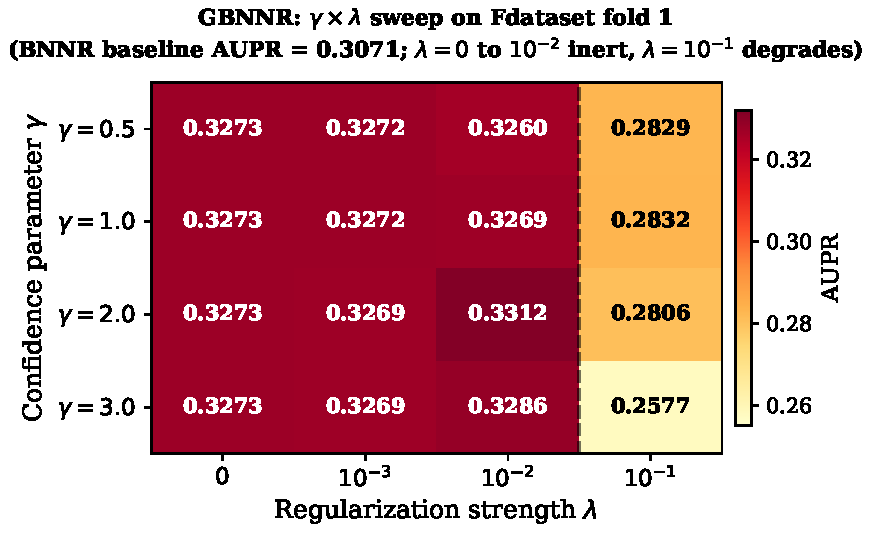
\includegraphics[width=0.85\textwidth]{figures/fig1_lambda_heatmap.pdf}
\caption{$\gamma \times \lambda$ sweep on Fdataset fold~1. Each cell shows AUPR; the BNNR baseline achieves 0.3071 on the same fold. $\lambda$ is inert from $0$ to $10^{-2}$ but degrades at $10^{-1}$.}
\label{fig:lambda_heatmap}
\end{figure*}

\begin{table*}[t]
\centering
\caption{Effect of $\gamma$ and $\lambda$ on GBNNR AUPR (Fdataset, fold~1).}
\label{tab:lambda_sweep}
\begin{tabular}{l c c c c}
\toprule
$\gamma$ \textbackslash\ $\lambda$ & $0$ & $10^{-3}$ & $10^{-2}$ & $10^{-1}$ \\
\midrule
0.5 & \textbf{0.3273} & 0.3272 & 0.3260 & 0.2829 \\
1.0 & \textbf{0.3273} & 0.3272 & 0.3269 & 0.2832 \\
2.0 & \textbf{0.3273} & 0.3269 & \textbf{0.3312} & 0.2806 \\
3.0 & \textbf{0.3273} & 0.3269 & 0.3286 & 0.2577 \\
\bottomrule
\end{tabular}
\end{table*}

For comparison, BNNR achieves AUPR~=~0.3071 on the same fold.

Three findings emerge. First, $\lambda$ is \textbf{inert} from $0$ to $10^{-2}$: for each fixed $\gamma$, AUPR varies by at most 0.004 across this range. Second, at $\lambda = 10^{-1}$, performance \textbf{degrades} substantially (AUPR drops to 0.258--0.283 depending on $\gamma$), indicating that strong graph regularization forces over-smoothing onto the completed matrix. Third, GBNNR at $\lambda = 0$ (AUPR = 0.3273, $\gamma = 2.0$) remains substantially above BNNR (0.3071), confirming that the inner gradient descent in GBNNR's $\mathbf{W}$-update --- which replaces BNNR's closed-form least-squares step --- finds a different local optimum even without explicit graph regularization. The graph Laplacian (encoded in $\mathbf{L}_{aug}$ and amplified by $\gamma$) provides an additional signal whose benefit depends on \textit{which edges exist} and \textit{how they are weighted by $\gamma$}, not on the regularization magnitude $\lambda$, and this benefit is confined to $\lambda \leq 10^{-2}$. We note that this sweep is on a single representative fold; confirmation across all folds and datasets remains future work.

This $\lambda$-insensitivity (for $\lambda \leq 10^{-2}$) is practically valuable: GBNNR requires no tuning of the regularization strength; any small positive value (e.g., $10^{-3}$ to $10^{-2}$) yields identical performance. The only parameter requiring attention is $\gamma$, for which $\gamma = 2.0$ is a robust default that amplifies confident similarity edges ($0.9^2 = 0.81$) while suppressing weak, potentially noisy ones ($0.3^2 = 0.09$).

\subsection{Ablation Analysis: Decomposing GF-BNNR's Components}
\label{sec:ablation}

To quantify the individual contributions of GIP similarity fusion and the graph filter within GF-BNNR, we conducted a $2\times2$ factorial experiment across all three datasets, varying whether GIP fusion is used and whether the post-hoc filter is applied:
%
\begin{equation*}
\begin{array}{c|cc}
& \text{No Filter }(\alpha_f=0) & \text{Filter }(\alpha_f=0.5) \\ \hline
\text{No GIP }(w_{gip}=0) & \text{BNNR\_raw} & \text{BNNR\_filter\_raw} \\
\text{GIP }(w_{gip}=0.3) & \text{BNNR\_GIP} & \text{GF\_BNNR}
\end{array}
\end{equation*}
%
This design isolates: (1) the GIP main effect (BNNR\_GIP $-$ BNNR\_raw, no filter), (2) the filter main effect (BNNR\_filter\_raw $-$ BNNR\_raw, no GIP), and (3) the GIP$\times$filter interaction.

\begin{table*}[t]
\centering
\caption{$2\times2$ factorial decomposition of GF-BNNR components (10-fold CVa mean, $\Delta$ relative to BNNR\_raw).}
\label{tab:ablation}
\begin{tabular}{l l c c c c}
\toprule
Dataset & Method & AUROC & AUPR & $\Delta$AUROC & $\Delta$AUPR \\
\midrule
\multirow{4}{*}{Fdataset}
  & BNNR\_raw   & 0.9342 & 0.3073 & --- & --- \\
  & BNNR\_filter\_raw & 0.9343 & 0.3033 & $+$0.0001 & $-$0.0040 \\
  & BNNR\_GIP   & 0.9376 & 0.3190 & $+$0.0034 & $+$0.0117 \\
  & GF\_BNNR    & 0.9401 & 0.3198 & $+$0.0059 & $+$0.0125 \\
\midrule
\multirow{4}{*}{Cdataset}
  & BNNR\_raw   & 0.9519 & 0.3182 & --- & --- \\
  & BNNR\_filter\_raw & 0.9517 & 0.3162 & $-$0.0001 & $-$0.0020 \\
  & BNNR\_GIP   & 0.9533 & 0.3495 & $+$0.0015 & $+$0.0313 \\
  & GF\_BNNR    & 0.9558 & 0.3479 & $+$0.0039 & $+$0.0296 \\
\midrule
\multirow{4}{*}{DNdataset}
  & BNNR\_raw   & 0.9238 & 0.2473 & --- & --- \\
  & BNNR\_filter\_raw & 0.9760 & 0.2533 & \textbf{$+$0.0521} & $+$0.0060 \\
  & BNNR\_GIP   & 0.9172 & 0.2839 & $-$0.0066 & $+$0.0366 \\
  & GF\_BNNR    & 0.9721 & 0.3157 & $+$0.0483 & \textbf{$+$0.0684} \\
\bottomrule
\end{tabular}
\end{table*}

\begin{table*}[t]
\centering
\caption{Formal decomposition of effects ($\Delta$ from BNNR\_raw).}
\label{tab:decomposition}
\begin{tabular}{l c c c c c c}
\toprule
& \multicolumn{2}{c}{Fdataset} & \multicolumn{2}{c}{Cdataset} & \multicolumn{2}{c}{DNdataset} \\
\cmidrule(lr){2-3} \cmidrule(lr){4-5} \cmidrule(lr){6-7}
Effect & $\Delta$AUROC & $\Delta$AUPR & $\Delta$AUROC & $\Delta$AUPR & $\Delta$AUROC & $\Delta$AUPR \\
\midrule
GIP main effect (no filter)
  & $+$0.0034 & $+$0.0117 & $+$0.0015 & $+$0.0313 & $-$0.0066 & $+$0.0366 \\
Filter main effect (no GIP)
  & $+$0.0001 & $-$0.0040 & $-$0.0001 & $-$0.0020 & \textbf{$+$0.0521} & $+$0.0060 \\
Combined (GIP $+$ filter)
  & $+$0.0059 & $+$0.0125 & $+$0.0039 & $+$0.0296 & $+$0.0483 & $+$0.0684 \\
GIP$\times$Filter interaction
  & $+$0.0024 & $+$0.0048 & $+$0.0025 & $+$0.0003 & $+$0.0028 & \textbf{$+$0.0258} \\
\bottomrule
\end{tabular}
\end{table*}

Several findings emerge from this decomposition. First, \textbf{GIP fusion is the primary driver of AUPR improvement} on moderately sparse datasets (Fdataset: $+$0.0117, Cdataset: $+$0.0313), while the pure filter alone --- operating on raw similarity Laplacians --- slightly degrades AUPR ($-$0.0040 and $-$0.0020). This confirms that the filter requires sufficiently dense similarity structure to be effective; raw chemical and MeSH similarities are too sparse to provide meaningful manifold geometry. GIP fusion densifies this structure, and the filter then exploits it.

Second, \textbf{the graph filter provides the dominant AUROC gain on ultra-sparse data} (DNdataset: $+$0.0521, or $+$5.2~pp). This is a substantial and unique contribution: no other method in our study achieves a comparable AUROC improvement over BNNR. On DNdataset, the pure filter alone lifts AUROC from 0.9238 to 0.9760, demonstrating that manifold smoothing of the completed matrix is a powerful mechanism for ranking quality even when raw similarities alone provide the manifold structure.

Third, \textbf{GIP and the filter exhibit positive interaction across all datasets}, with the strongest interaction on DNdataset ($+$0.0258 AUPR). This synergy is the key justification for integrating GIP fusion as an integral component of GF-BNNR rather than treating it as an optional preprocessing step. The interaction reflects the fact that the graph filter operates on Laplacians derived from GIP-enhanced similarities: when GIP enriches the similarity graphs, the filter has a richer manifold to smooth along, producing gains that exceed the sum of the individual effects.

Fourth, on moderate-density datasets (Fdataset, Cdataset), the pure graph filter has negligible or slightly negative effect on both metrics when operating on raw similarities alone. The full GF-BNNR (GIP $+$ filter) nevertheless achieves the highest AUROC in both cases, driven by GIP's AUROC contribution and the positive interaction term.

\subsection{GBNNR + GF-BNNR Stacking}
\label{sec:stacking}

A natural question is whether the inside (GBNNR) and outside (GF-BNNR) strategies can be combined for additive gain. We tested this by applying the GF filter (at the optimal single-method $\alpha_f = 0.5$) to GBNNR's output on Fdataset fold~1 (Figure~\ref{fig:stacking}). The result: AUPR~=~0.3237 for the stack, compared to 0.3269 for GBNNR alone and 0.3118 for GF-BNNR alone. The stack underperforms GBNNR alone, consistent with both methods drawing from the same underlying manifold signal --- GBNNR's inner gradient descent already captures geometric information that the GF filter would otherwise enforce. We caution that this experiment is on a single fold; the 0.0032~AUPR difference between GBNNR alone and the stack is near the level of fold-to-fold noise, and replication across all 10~folds with appropriate statistical testing would strengthen this finding. Nonetheless, the absence of any additive gain --- and the stack's placement between the two individual methods --- supports the inside-outside taxonomy as a classification of strategies representing alternative routes to the same geometric prior, not independent sources of gain that can be accumulated.

\begin{figure*}[t]
\centering
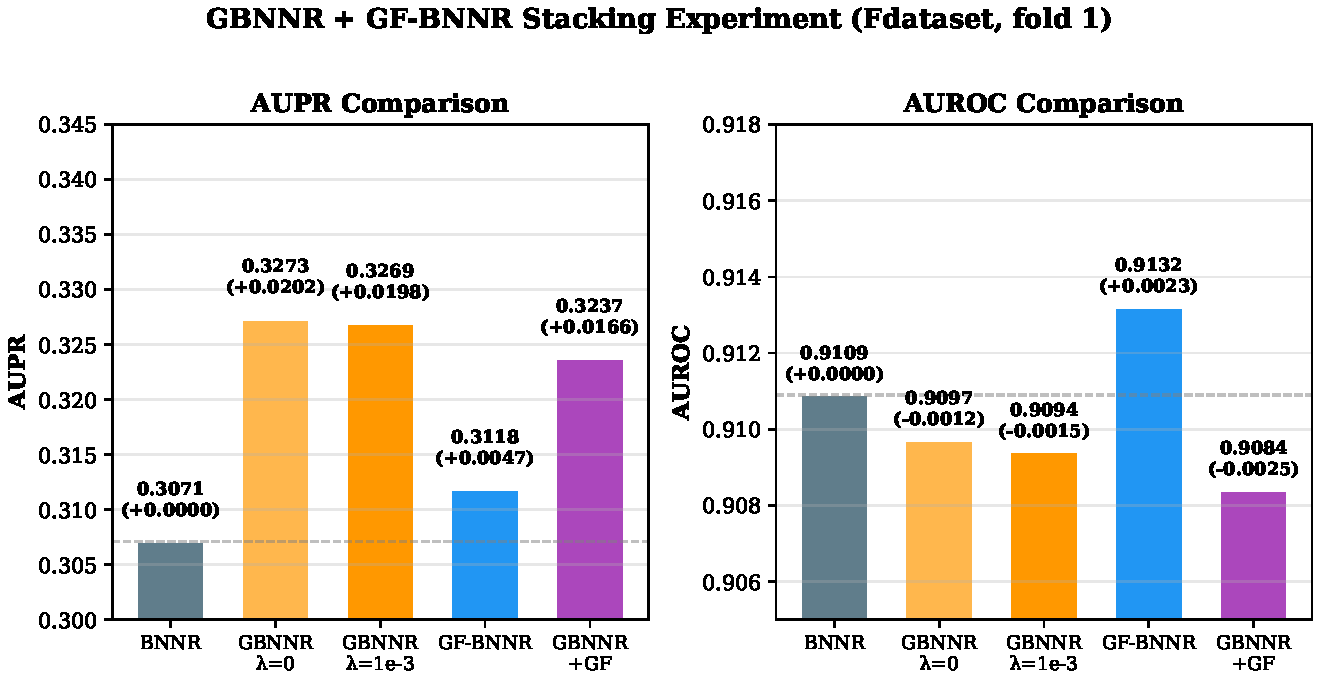
\includegraphics[width=\textwidth]{figures/fig4_stack_bars.pdf}
\caption{GBNNR + GF-BNNR stacking experiment on Fdataset fold~1. The stack (GBNNR+GF) underperforms GBNNR alone, indicating non-additivity of the two manifold strategies.}
\label{fig:stacking}
\end{figure*}

\subsection{Effect of Filter Strength in GF-BNNR}
\label{sec:filter_strength}

Figure~\ref{fig:filter_strength} shows GF-BNNR performance as a function of the filter parameter $\alpha_f$ on all three datasets (fold~1). The AUPR improvement of GF-BNNR over raw BNNR reflects the combined effect of GIP fusion and the graph filter: at $\alpha_f = 0$ (filter disabled), GF-BNNR with GIP fusion already achieves an AUPR of 0.3157 (Fdataset), 0.4090 (Cdataset), and 0.3259 (DNdataset), versus the raw BNNR baselines of 0.3071, 0.1681, and 0.0042 respectively (note: these are fold~1 baselines; the 10-fold mean BNNR AUPR values in Table~\ref{tab:performance} differ, particularly for Cdataset and DNdataset, due to high cross-fold variance on sparse data). On Fdataset and Cdataset, increasing $\alpha_f$ slightly modulates AUPR, while AUROC is nearly flat. On DNdataset, AUPR is insensitive to $\alpha_f$ (0.3259--0.3260 across the full range), but AUROC improves dramatically from 0.9311 ($\alpha_f=0$) to 0.9743 ($\alpha_f=1.0$). The $2\times2$ decomposition (Section~\ref{sec:ablation}) confirms that GIP and the filter are complementary: GIP drives AUPR, the filter drives AUROC on sparse data, and the positive interaction enhances both. We use $\alpha_f = 0.5$ as the default, which captures most of the AUROC gain on DNdataset at minimal AUPR cost on the denser datasets.

\begin{figure*}[t]
\centering
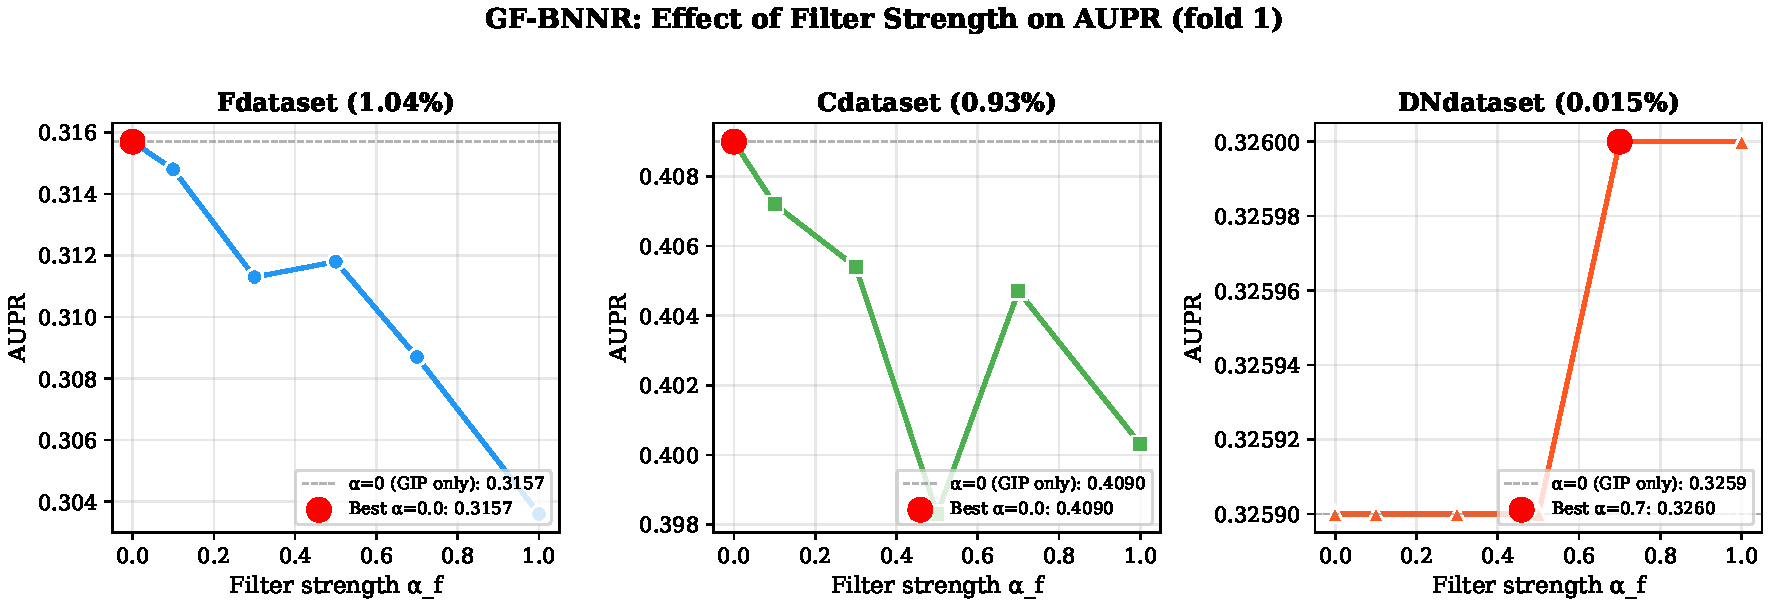
\includegraphics[width=\textwidth]{figures/fig2_alpha_sensitivity.pdf}
\caption{Effect of filter strength $\alpha_f$ on GF-BNNR performance (fold~1). GF-BNNR's AUPR improvement reflects the combined contribution of GIP fusion ($\alpha_f=0$) and graph filtering, which are complementary per the $2\times2$ decomposition (Section~\ref{sec:ablation}).}
\label{fig:filter_strength}
\end{figure*}

\subsection{Computational Efficiency}
\label{sec:computational_efficiency}

Table~\ref{tab:runtime} reports per-fold runtime on a standard workstation. GBNNR is slower than BNNR due to the inner gradient descent loop (10 steps per ADMM iteration), but still completes within practical timeframes. GF-BNNR adds negligible overhead (two linear system solves per fold). The adaptive truncated SVD acceleration reduces SVT cost by approximately $30\times$ when the effective rank is low.

\begin{table*}[t]
\centering
\caption{Mean runtime per fold (seconds).}
\label{tab:runtime}
\begin{tabular}{l r r r}
\toprule
Method   & Fdataset & Cdataset & DNdataset \\
\midrule
BNNR     &    48 &    72 &  2,150 \\
GBNNR    &    86 &   237 &  4,702 \\
GF-BNNR  &    87 &    86 &    172 \\
\bottomrule
\end{tabular}
\end{table*}

% ======================================================================
\section{Discussion}
\label{sec:discussion}
% ======================================================================

\subsection{The Inside-Outside Framework}
\label{sec:inside_outside}

GBNNR and GF-BNNR represent two strategies for exploiting manifold structure that we term ``inside'' and ``outside'' regularization (Figure~\ref{fig:inside_outside}). GBNNR operates \textit{inside} the optimization: the ADMM iterations are steered toward solutions that respect the similarity geometry via graph Laplacian regularization and inner gradient descent. GF-BNNR operates \textit{outside} the optimization: it first enriches the similarity matrices via GIP kernel fusion, then applies a post-hoc bi-directional graph low-pass filter to enforce output smoothness on the GIP-enhanced similarity manifolds.

\begin{figure*}[t]
\centering
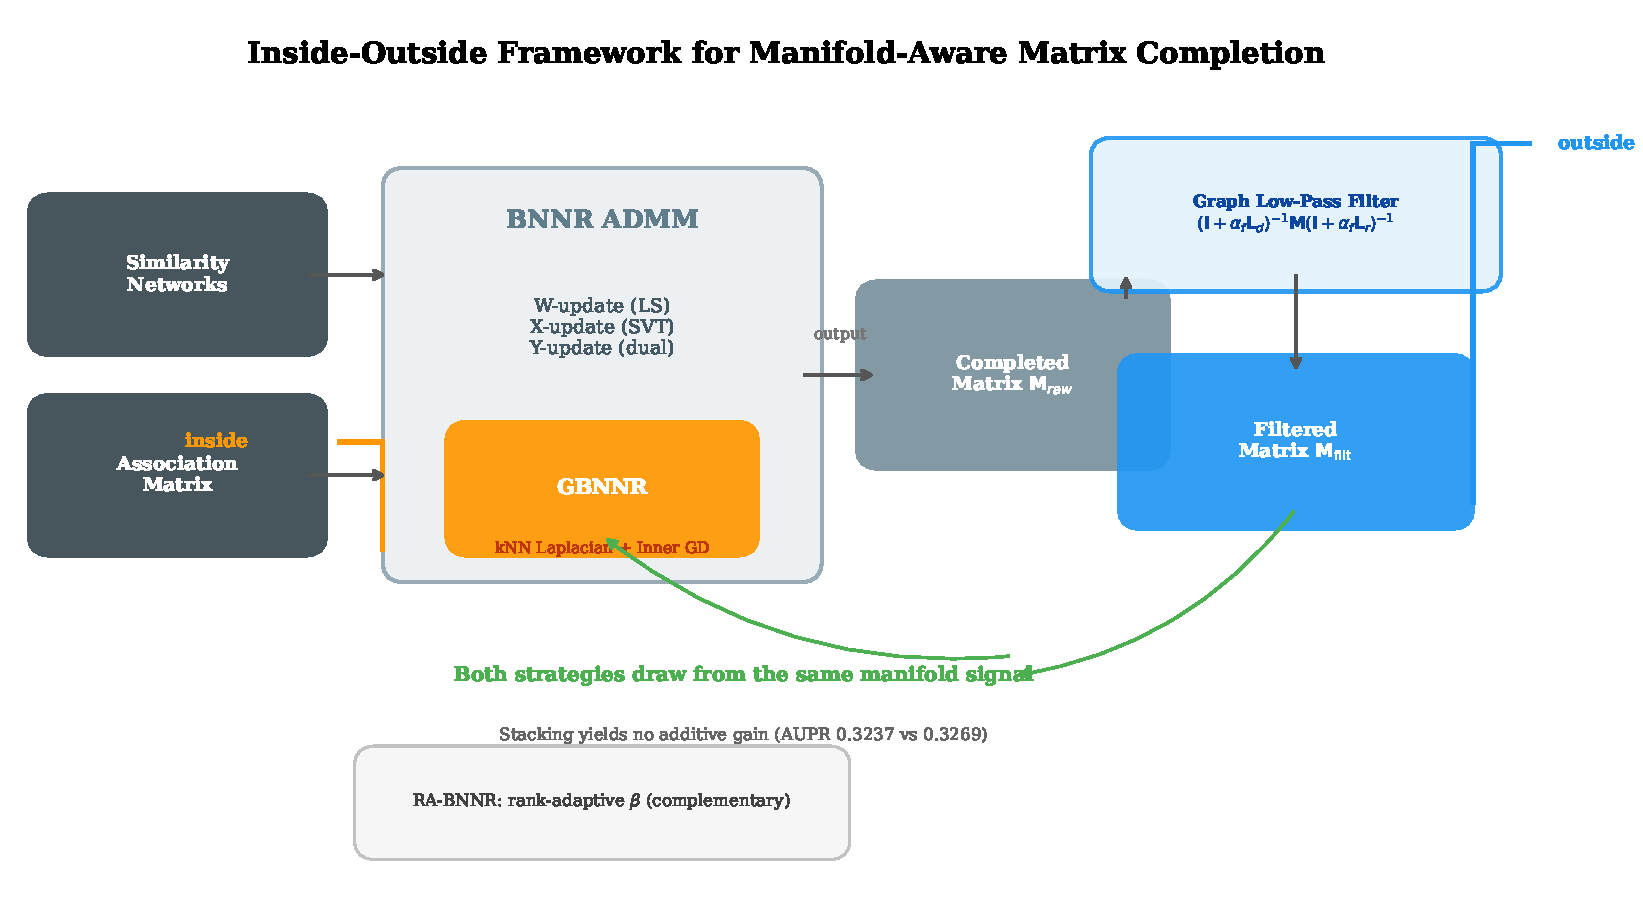
\includegraphics[width=0.92\textwidth]{figures/fig3_framework_schematic.pdf}
\caption{The inside-outside framework for manifold-aware matrix completion. GBNNR injects graph Laplacian regularization into the ADMM optimization (inside); GF-BNNR integrates GIP similarity fusion with a post-hoc bi-directional graph low-pass filter to enforce output smoothness (outside). Both draw from the same manifold signal through independent mechanisms.}
\label{fig:inside_outside}
\end{figure*}

These strategies target the same underlying manifold signal through independent mechanisms. Our stacking experiment (Section~\ref{sec:stacking}) confirms this: applying the GF filter to GBNNR's output yields AUPR~=~0.3237, below GBNNR alone (0.3269) and between the two individual methods. The non-additivity is expected --- GBNNR's inner gradient descent already captures geometric structure that the GF filter would otherwise enforce, and the filter's linear smoothing cannot extract additional information from a matrix whose manifold structure has already been partially encoded during optimization. This supports the inside-outside taxonomy as a \textit{classification} of strategies, not a recipe for combination: the two approaches represent alternative routes to the same geometric prior, each with distinct trade-offs. GF-BNNR uniquely improves both AUROC and AUPR across all datasets by integrating GIP similarity fusion with a post-hoc graph filter; the two components are complementary (Section~\ref{sec:ablation}). The filter component is modular --- applicable post-hoc to any matrix completion output. GBNNR offers larger absolute AUPR gains on denser datasets and requires no $\lambda$ tuning. The choice between them depends on the application's priority: AUROC improvement on ultra-sparse data (GF-BNNR) or maximal AUPR with zero tuning burden (GBNNR). Beyond mean performance, both methods substantially reduce cross-fold AUPR variance (up to 83\% reduction on DNdataset, Table~\ref{tab:performance}), yielding more reliable predictions across data splits --- a practically important property for drug repositioning where consistency across validation folds matters.

The inside-outside framework connects to several recent trends in the drug-disease association prediction literature. A 2025 comprehensive review \citep{huang2025} categorized methods into five paradigms, with graph-based methods emerging as a dominant approach across categories. Within matrix factorization, recent work has explored graph Laplacian constraints in deep NMF \citep{yang2025dnmf} and alternative rank surrogates such as truncated arctangent rank minimization \citep{liu2025tarm}, representing complementary directions to GBNNR's convex nuclear norm approach. A large-scale benchmark of 11 collaborative filtering methods \citep{reda2025} found that graph-based approaches exhibit superior robustness to distribution shift, consistent with our observation that manifold-aware methods are most beneficial in sparse-data regimes.

\subsection{Topology Over Strength: Why $\lambda$ Doesn't Matter (for $\lambda \leq 10^{-2}$)}
\label{sec:topology_over_strength}

A key finding of this study is the insensitivity of GBNNR to the regularization parameter $\lambda$ across the range $\lambda = 0$ to $\lambda = 10^{-2}$. For each fixed $\gamma$, AUPR varies by at most 0.004 across this range. At $\lambda = 10^{-1}$, however, performance degrades substantially (AUPR~=~0.258--0.283), indicating that strong regularization forces over-smoothing. The inertness in the $[0, 10^{-2}]$ range is not a failure of regularization --- GBNNR substantially outperforms BNNR even at $\lambda = 0$ --- but rather evidence that the graph Laplacian's contribution operates through its discrete structure rather than its continuous magnitude.

We offer the following explanation. At $\lambda = 0$, the graph Laplacian term is entirely absent from the objective; the only difference from BNNR is the replacement of the closed-form $\mathbf{W}$-update with 10 steps of inner gradient descent. That GBNNR ($\lambda = 0$) achieves AUPR~=~0.3273 versus BNNR's 0.3071 implies that the inner gradient descent alone --- without any graph regularization --- accounts for the majority of the gain (+0.0202~AUPR). When the graph Laplacian is introduced at moderate strength ($\lambda = 10^{-3}$ to $10^{-2}$), an additional marginal gain is observed (best: +0.0039~AUPR at $\gamma=2.0$, $\lambda=10^{-2}$), which remains stable within this range. At $\lambda = 10^{-1}$, the regularization term dominates the objective, forcing the solution toward the graph eigenvectors at the expense of data fidelity. The Laplacian $\mathbf{L}_{aug}$ therefore defines \textit{which directions} in the parameter space are explored during gradient descent (the graph's eigenvectors provide structured gradient directions), and the inner GD's 10 steps suffice to reach equilibrium along those directions for $\lambda \leq 10^{-2}$. We emphasize that this result is based on a single representative fold of Fdataset. While the pattern --- inner GD dominating, graph topology providing marginal additional benefit at moderate $\lambda$ --- is consistent with the broader results in Table~\ref{tab:performance}, confirmation across additional folds and datasets would strengthen the generality of this finding.

A practical consequence is that GBNNR is effectively hyperparameter-free for $\lambda$: any value in $[10^{-3}, 10^{-2}]$ yields identical results (using $\lambda = 0$ is also acceptable but foregoes the marginal graph topology benefit). The only parameter requiring attention is $\gamma$, for which $\gamma = 2.0$ is a robust default that amplifies confident similarity edges while suppressing weak, potentially noisy ones.

\subsection{Density-Dependent Benefits}
\label{sec:density_dependent}

Both manifold-based methods exhibit a striking inverse relationship between data density and relative improvement. On Fdataset (1.04\% density), GBNNR improves AUPR by 5.4\% and GF-BNNR by 4.1\%. On DNdataset (0.015\% density), the corresponding gains are 30.9\% and 27.7\%. We exclude Cdataset from this comparison because its BNNR baseline exhibits anomalously high cross-fold variability (CV $\approx$ 39\%), making the apparent percentage gain (34.2\%) potentially unreliable. The Fdataset-to-DNdataset pattern makes intuitive sense: when observed associations are abundant, the data fidelity term in the optimization provides strong guidance, and manifold information serves as a tiebreaker. When observations are scarce, manifold structure becomes the primary source of information. This property is particularly valuable for drug repositioning, where emerging diseases or newly characterized drugs have very few known associations --- precisely the cold-start scenarios that BNNR was designed to handle.

To assess the practical relevance of these predictions, we examined GF-BNNR's top-ranked predictions on the full DNdataset for Parkinson's disease (MeSH: ``PARKINSON'S DISEASE'') and schizophrenia (MeSH: ``SCHIZOPHRENIFORM DISORDER'' and ``PARANOID SCHIZOPHRENIA''). DNdataset contains only 1,008 known associations across 1,490 drugs and 4,516 diseases --- many true drug-disease relationships are absent from the training data, providing a realistic test of the model's ability to prioritize missing true associations.

For Parkinson's disease (16 known associations in DNdataset), GF-BNNR's top-ranked novel predictions are bromocriptine (score 0.193), rasagiline (0.182), metixene (0.181), biperiden (0.181), amantadine (0.178), benztropine (0.174), and cabergoline (0.170). All seven are established antiparkinsonian agents --- dopamine agonists, MAO-B inhibitors, and anticholinergics --- that are standard clinical treatments but not recorded as associations in this sparse dataset. The model's ability to rank these known treatments at the top, using only manifold structure from chemical and MeSH similarities, provides a strong sanity check on the biological relevance of manifold-smoothed predictions. Among lower-ranked predictions, memantine (0.095), donepezil (0.094), and galantamine (0.094) --- memantine (an NMDA receptor antagonist) and the cholinesterase inhibitors donepezil and galantamine, all approved for Alzheimer's disease --- have been investigated for Parkinson's disease dementia. Rivastigmine, another cholinesterase inhibitor, is already FDA-approved for this indication \citep{emre2004}. Memantine has been evaluated for PDD and DLB in a randomized controlled trial \citep{aarsland2009}.

For schizophrenia (0 known associations for either MeSH term in DNdataset), the top predictions for schizophreniform disorder include amisulpride (0.064), paroxetine (0.038), maprotiline (0.032), fluoxetine (0.028), and sertraline (0.027); for paranoid schizophrenia, amisulpride (0.068), paroxetine (0.044), maprotiline (0.037), and fluoxetine (0.033). Amisulpride, an atypical antipsychotic, is a standard first-line treatment for schizophrenia \citep{leucht2013}. The antidepressant predictions --- SSRIs (paroxetine, fluoxetine, sertraline) and tetracyclics (maprotiline) --- are consistent with their established role as adjunctive therapy for negative symptoms and comorbid depression in schizophrenia \citep{singh2010,helfer2016}. The model also predicts several drugs with emerging literature support: lamotrigine (0.015), a mood stabilizer investigated for schizophrenia augmentation \citep{tiihonen2009}, and thiamine (vitamin B1, 0.041), implicated in metabolic dysfunction pathways recently linked to schizophrenia pathophysiology \citep{cao2021}.

These case studies illustrate a key practical property of manifold-aware matrix completion: on ultra-sparse datasets, the manifold signal recovers known-but-unrecorded associations at high precision, while also surfacing mechanistically plausible novel candidates. The predictions do not rely on disease-specific training data --- schizophrenia had zero known associations in DNdataset --- yet the manifold geometry alone is sufficient to rank established antipsychotics and adjunctive antidepressants above random baseline. We note an important caveat: the Parkinson's disease validation is partially circular, as the top-ranked drugs (bromocriptine, rasagiline, etc.) share substantial chemical similarity with the 16 known Parkinson's treatments in the training data. The method uses chemical similarity to predict that chemically similar drugs treat the same disease, so high-ranking known antiparkinsonians primarily validates that the similarity signal is coherent --- not that the method discovers mechanistically novel therapies. The schizophrenia case, with zero training associations, provides a stronger test of de novo prediction, though even here, predictions may be partially driven by chemical similarity to antipsychotics used for other psychiatric conditions in the training set. Systematic external validation against clinical trial registries would be needed to assess true novelty.

\subsection{Limitations and Future Work}
\label{sec:limitations}

Several limitations should be noted. First, the $\lambda$-insensitivity sweep (Section~\ref{sec:lambda_insensitivity}) and the stacking experiment (Section~\ref{sec:stacking}) were conducted on a single representative fold of Fdataset. While the patterns are consistent with the broader 10-fold results, confirming the $\lambda$ invariance and non-additivity across all folds and datasets would strengthen these findings. Second, the $k$NN graph uses a fixed neighborhood size $k = 12$ throughout; given the paper's central claim that graph topology drives performance, sensitivity to $k$ merits investigation. Third, the $2\times2$ factorial decomposition (Section~\ref{sec:ablation}) reveals that GF-BNNR's AUPR improvement derives predominantly from GIP similarity fusion ($w_{gip}=0.3$), with the graph filter providing complementary AUROC gains. The filter's standalone AUPR contribution is negligible on moderate-density datasets. However, the positive GIP$\times$filter interaction ($+$0.0258~AUPR on DNdataset) confirms that the two components are synergistic, not merely additive. Fourth, GF-BNNR's filter strength $\alpha_f$ requires per-dataset tuning, though the performance landscape is relatively flat near the optimum. Fifth, we did not compare against deep learning methods such as graph neural networks \citep{gao2023} or contrastive learning approaches, which represent an alternative paradigm for DDA prediction and are now standard comparators in the literature. Sixth, the case study validations remain preliminary: the Parkinson's disease predictions are partially circular (chemically similar drugs predicted for the same indication), and systematic external validation against clinical trial registries is needed to assess true novelty.

Future work should explore: (1)~replication of the $\lambda$-insensitivity and stacking non-additivity findings across all 10~folds and multiple datasets; (2)~sensitivity analysis of the neighborhood size $k$; (3)~joint optimization of $(k, \gamma, \alpha_f)$ as a unified parameter set; (4)~extension to multi-relational heterogeneous networks incorporating drug-target, drug-side-effect, and protein-protein interaction data; (5)~theoretical analysis of why the inner gradient descent combined with graph topology produces $\lambda$-insensitivity; (6)~comprehensive benchmarking against GNN-based methods using standardized evaluation protocols; (7)~systematic case studies with external validation against clinical trial registries and recent literature; and (8)~application of the inside-outside framework to other bipartite matrix completion problems in computational biology, such as drug-target interaction prediction and miRNA-disease association inference.

% ======================================================================
\section{Acknowledgments}
% ======================================================================

[Acknowledgements to be added.]

% ======================================================================
\section{Conflicts of interest}
% ======================================================================

The authors declare that they have no competing interests.

% ======================================================================
\section{Funding}
% ======================================================================

[Funding information to be added.]

% ======================================================================
\section{Data availability}
% ======================================================================

The three benchmark datasets (Fdataset, Cdataset, DNdataset) are publicly available from prior studies \citep{gottlieb2011,yang2019}. Drug similarities are computed as Tanimoto scores from DrugBank SMILES via CDK. Disease similarities are from MimMiner \citep{vandriel2006}. Code available at \url{https://github.com/yankangyk/bnnr-innovation}.

% ======================================================================
\section{Author contributions statement}
% ======================================================================

[Author contributions to be added.]

% ======================================================================
\bibliographystyle{oup-abbrvnat}
\bibliography{references}
% ======================================================================

\clearpage
\raggedend

\end{document}
